\documentclass{beamer}

\usetheme{Boadilla}

\usepackage[utf8]{inputenc}
\usepackage[francais]{babel}
\usepackage{multicol} % itemize sur plusieurs colonnes
\usepackage{tikz} % pour superposer les images
\usepackage{subfig} % pour mettre images à côté
\setcounter{tocdepth}{1} % afficher que les sections dans le sommaire

\hypersetup{ % couleur des liens
    colorlinks=true,
    linkcolor=blue,
    filecolor=black,      
    urlcolor=blue,
}

\AtBeginSection[] % faire apparaître le sommaire avant chaque nouvelle section
{
  \begin{frame}
    \frametitle{Sommaire}
    \tableofcontents[currentsection]
  \end{frame}
}

\newif\ifplacelogo %Booléen pour placer ou non le logo
\placelogotrue %Initialisation booléen à 'True'
\logo{\ifplacelogo\includegraphics[height=5mm]{Images/logoINSA.png}\fi} %Initialisation du logo (fonction du booléen)

\title{Test de Tukey (LSD)}
\author[MA \--- DT]{ABOUZAID Mehdi \\ TOOMEY Damien}
\institute[INSA Rouen]{INSA \--- Institut National des Sciences Appliquées de Rouen}
\date{\today}

\begin{document}

\begin{frame}
\titlepage
\end{frame}

\placelogofalse
\begin{frame}
\frametitle{Sommaire} 
\tableofcontents
\end{frame}	

\section{Base de données}

\begin{frame}
\frametitle{Base de données}

Temps d'un sprint (en secondes) sur 35 mètres 

\begin{center}
\begin{tabular}{r@{}c}    
  33 athlètes par colonne & $\left\{
\begin{tabular}{ |c|c|c| }
\hline
Non fumeur & Ancien fumeur & Fumeur actuel \\ 
\hline
7.9780 & 7.4430 & 7.3120 \\
\hline  
8.0040 & 7.0250 & 6.4990 \\
\hline  
4.6500 & 7.7060 & 7.0130 \\   
\hline  
4.7500 & 5.5370 & 7.4940 \\   
\hline
... & ... & ... \\    
\hline  
4.8730 & 6.2330 & 8.2320 \\  
\hline
\end{tabular}
  \right.\kern-\nulldelimiterspace$
\end{tabular}
\end{center}

\end{frame}

\section{Analyse de la variance (ANOVA)}

\subsection{Les limites du test de Student}
\begin{frame}
\frametitle{Les limites du test de Student}
Utilisé pour comparer soit :
\begin{itemize}
\item[•] deux variables quantitatives
\item[•] une variable quantitative et une variable qualitative \\
\end{itemize}

\begin{exampleblock}{Exemple d'hypothèses du test de Student :}
\[\left\{\begin{array}{ll}
H_0 : \mu_1 = \mu_2 \\
H_1 : \mu_1 \neq \mu_2 \\
\end{array}\right. \]
\end{exampleblock}

\begin{alertblock}{Inflation de $\alpha$}
$\dbinom{c}{2}$ tests de Student  $\rvert$
Pour $c=5 \Rightarrow \dbinom{5}{2}=10$ tests de Student \\~\\
Au départ, $\alpha=0.05$ pour chaque test mais 10 tests de Student sur le même jeu de données entraîne $ \alpha'= 1 - (1 - \alpha)^{10} = 0.40$ \\
Soit 40\% de risque de faire une erreur de type 1 sur les 10 tests menés 
\end{alertblock}
\end{frame}

\subsection{L'ANOVA : une généralisation du test de Student}
\begin{frame}
\frametitle{L'ANOVA : une généralisation du test de Student}
 
\begin{block}{Remarque}
L'ANOVA (analysis of variance) permet d'éviter cette inflation de $\alpha$
\end{block}

Il existe différents types d'ANOVA et d'autres variantes :
\begin{multicols}{2}
\begin{itemize}
\item[•] {\only<2>{\color{red}}ANOVA à un facteur}
\item[•] ANOVA à deux facteurs
\item[•] ...
\item[•] ANOVA à n facteurs
\item[•] ANCOVA
\item[•] MANOVA
\item[•] MANCOVA
\end{itemize}
\end{multicols}

\begin{alertblock}{But de notre étude :  les tests a posteriori}
Ils ne sont réalisés que si l'on rejette $H_0$ à la suite d'une ANOVA
\begin{itemize}
\item[•] test de Fisher (LSD)
\item[•] test de Tukey (HSD)
\end{itemize} 
\end{alertblock}
\end{frame}

\subsection{Les conditions d'application de l'ANOVA à un facteur}
\begin{frame}

\begin{alertblock}{Remarque : ANOVA \underline{à un facteur}}
On ne prend en compte qu'un seul facteur de variabilité
\end{alertblock}

\begin{itemize}
\frametitle{Les conditions d'application de l'ANOVA à un facteur (1/3)}
\item[I] la variable quantitative est continue
\item[II] au moins deux variables qualitatives
\item[] (identique au test de Student si on en a exactement deux)
\item[III] chaque groupe analysé est indépendant des autres groupes
\end{itemize} 

\begin{center}
\begin{tabular}{ |c|c|c| }
\hline
Non fumeur & Ancien fumeur & Fumeur actuel \\ 
\hline
7.9780 & 7.4430 & 7.3120 \\
\hline  
8.0040 & 7.0250 & 6.4990 \\
\hline  
4.6500 & 7.7060 & 7.0130 \\   
\hline  
4.7500 & 5.5370 & 7.4940 \\   
\hline
... & ... & ... \\    
\hline  
4.8730 & 6.2330 & 8.2320 \\  
\hline
\end{tabular}
\end{center}

\end{frame}

\begin{frame}
\frametitle{Les conditions d'application de l'ANOVA à un facteur (2/3)}

\begin{itemize}
\item[IV] pas de valeur aberrante
\end{itemize} 

\begin{figure}[H]
%\caption{}
\centerline{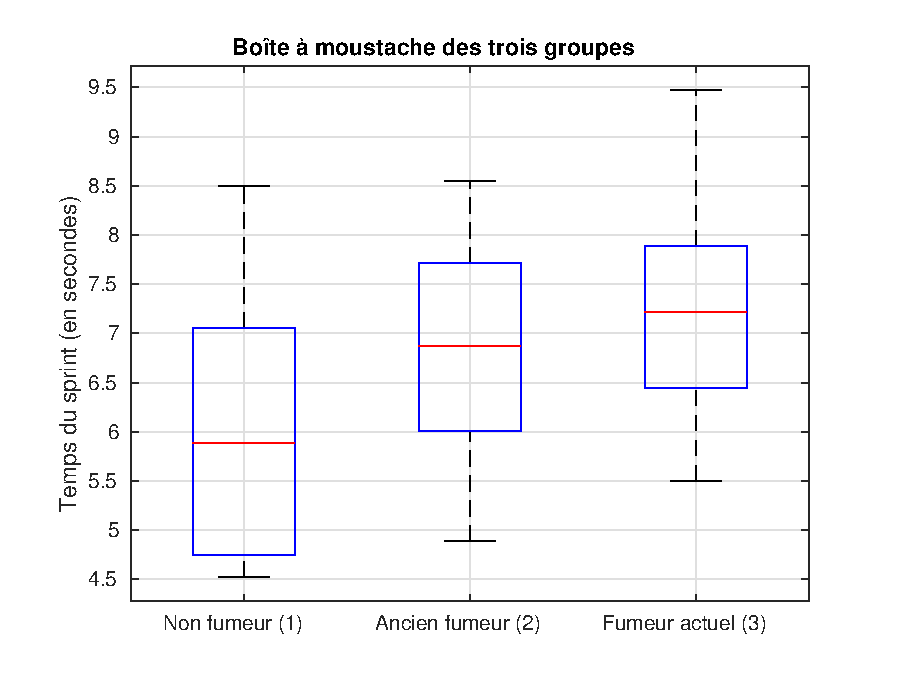
\includegraphics[width=9cm]{Images/BoiteAMoustachesParGroupe}}
\label{1}
\end{figure}
\end{frame}

\begin{frame}
\frametitle{Les conditions d'application de l'ANOVA à un facteur (3/3)}
\begin{itemize}
\item[V] les groupes suivent une loi normale  \\
\item[] (fonction \emph{chi2gof}) \\
\item[]
\item[VI] les variances sont les mêmes dans chaque groupe \\
\item[] (fonction \emph{vartestn})
\end{itemize} 
\end{frame}

% Diapositive pas prise en compte
\begin{frame}<presentation:0>[noframenumbering]
\frametitle{Les conditions d'application de l'ANOVA à un facteur (3/4)}
\begin{itemize}
\item[•] les groupes suivent une loi normale \\
\end{itemize} 
\phantom{newline}

Fonction \emph{chi2gof} de Matlab (Chi-square goodness-of-fit test)
\[ \left\{\begin{array}{ll}
H_0 : \text{les données suivent une distribution normale} \\
H_1 : \text{les données ne suivent pas une distribution normale}
\end{array}\right. \]

\phantom{newline}

$chi2gof = 1$ si le test rejette $H_0$ \\
$chi2gof = 0$ sinon \\

\phantom{newline}

Ici $chi2gof = 0$ donc $H_0$ est validée \\

\end{frame}

% Diapositive pas prise en compte
\begin{frame}<presentation:0>[noframenumbering]
\frametitle{Les conditions d'application de l'ANOVA à un facteur (4/4)}
\begin{itemize}
\item[•] les variances sont les mêmes dans chaque groupe \\
\end{itemize} 

Fonction \emph{vartestn} de Matlab (test de Bartlett)
\[ \left\{\begin{array}{ll}
H_0 : \text{chaque colonne de la matrice suit une distribution normale avec} \\
\quad \;\;\; \text{la même variance} \\
H_1 : \text{au moins une colonne de la matrice n'a pas la même variance} \\
\qquad \text{que les autres colonnes}
\end{array}\right. \]

On regarde la p-valeur pour savoir quelle hypothèse on valide \\
\begin{itemize}
\item[] $p-valeur > \alpha \Rightarrow H_0 \; \text{validée}$ \\
\item[] $p-valeur < \alpha \Rightarrow H_1 \; \text{validée}$ \\
\end{itemize} 

\phantom{newline}

Ici la $p-valeur=0.4271 > \alpha = 0.05$ donc on $H_0$ est validée
\end{frame}

\subsection{Les hypothèses de l'ANOVA à un facteur}
\begin{frame}
\frametitle{Les hypothèses de l'ANOVA à un facteur}

\begin{align*}
& \;\;\;\;\; \left\{\begin{array}{ll}
H_0 : \mu_1 = \mu_2 = ... = \mu_c \quad \text{(c : nombre de groupes)} \\ 
H_1 : \exists \; (i,j) \in  [\![1 ~;~ c]\!] ^2 \; \text{tel que} \; \mu_i \neq \mu_j
\end{array}\right. \\
& \\
& \Leftrightarrow \left\{\begin{array}{ll}
H_0 : \text{les moyennes de chaque groupe sont égales} \\
H_1 : \text{il existe au moins une moyenne qui n’est pas égale aux autres} \\
\end{array}\right.
\end{align*}
\end{frame}

\subsection{La définition du modèle}
\begin{frame}
\frametitle{Définition du modèle}
On choisit le modèle suivant :
\[ y_{ij}=\mu_i+\epsilon_{ij} \]

$i= 1...c$ (c : nombre de groupes) \\
$j= 1...r$ (r : effectif de chaque groupe)
\end{frame}

\subsection{Partie mathématique}
\begin{frame}
\frametitle{Partie mathématique (1/2)}

L'ANOVA se base sur deux types de variance :
\begin{itemize}
\item[•] variance expliquée (inter-classes) : 
\item[]résume la variabilité entre les classes (traitement et hasard)
\item[•] variance résiduelle (intra-classe) : 
\item[] résume la variabilité à l'intérieur des classes (hasard)
\end{itemize}

\begin{block}{Décomposition de la variance (de la $SCE_T$ plus précisément)}
\[\color{red} SCE_T \color{black} = \underbrace{SCE_F}_{\text{inter-classes (due au facteur)}} \color{black} + \color{blue} \underbrace{SCE_R}_{\text{intra-classe (résiduelle)}} \]
\href[pdfnewwindow]{../DecompositionDeLaVariance/decompositionVariance.pdf}{Démonstration}
\end{block}

\begin{block}{Degrés de liberté associés}
\begin{center}
$ \color{red} n-1 \color{black} = c-1 \color{black} + \color{blue} n-c $  
\end{center}         
\end{block}

\setlength{\columnsep}{-20pt}
\begin{multicols}{2}
\begin{itemize}
\item[•] c : nombre de groupes
\item[•] n : effectif total
\item[•] SCE : somme des carrés des écarts \\
\end{itemize}
\end{multicols}

\end{frame}

\begin{frame}
\frametitle{Partie mathématique (2/2)}

\begin{block}{L'ANOVA utilise la loi de Fisher}
\[ F_{observe} = \frac{\frac{SCE_F}{c-1}}{\frac{SCE_R}{n-c}}=\frac{CM_F}{CM_R} \]
\end{block}

\begin{itemize}
\item[] SCE : somme des carrés des écarts \\
\item[] CM : carré moyen \\
\end{itemize}

\begin{itemize}
\item[•] $F_{observe} < F_{tables} \Rightarrow $ acceptation de $H_0$
\item[•] $F_{observe} \ge F_{tables} \Rightarrow $ rejet de $H_0$
\end{itemize}

%On résume les calculs de l'ANOVA dans un tableau de la forme suivante :
%\begin{center}
%\begin{tabular}{ |c|c|c|c|c|c| }
%\hline
%Source & SCE & DDL & CM & F & $Prob>F$\\ 
%\hline
%Inter-classes & $SCE_F$ & $c-1$ & $CM_F$ & $F_{observe}$ & p-value\\
%\hline  
%Intra-classe & $SCE_R$ & $n-c$  & $CM_R$ & & \\
%\hline
%Total & $SCE_T$ & $n-1$ & & & \\
%\hline
%\end{tabular}
%\end{center}
\end{frame}

\subsection{Les résultats de l'ANOVA}
\begin{frame}
\frametitle{Les résultats de l'ANOVA}

\begin{align*}
& F_{observe} = 10.3687 \ge F_{tables}=3.09 \; \text{donc on rejette} \; H_0 \\
& p-valeur=8.3744 \cdot 10^{-5} < \alpha=0.05 \; \text{ce qui conforte le rejet de} \; H_0 
\end{align*}

\begin{figure}[H]
%\caption{}
    \begin{tikzpicture}
    \node(a){\centerline{\includegraphics[width=0.8\textwidth]{Images/TableauAnovaAlaMain}}};
    \node at (a.south)
    [
    anchor=center,
    xshift=0mm,
    yshift=7mm
    ]
    {
        \centerline{\includegraphics[width=0.8\textwidth]{Images/TableauAnovaMatlab}}
    };
    \end{tikzpicture}
\end{figure}
\end{frame}

\section{Test de Fisher (LSD : Least Significant Difference)}

\subsection{Test de Fisher (LSD) : Partie mathématique}
\begin{frame}
	\frametitle{Test de Fisher (LSD) : Partie mathématique}
	
	Rejet de $H_0 \Rightarrow$ déterminer les groupes qui diffèrent en comparant les moyennes des groupes deux à deux \\
	
\begin{alertblock}{Fisher établit le test LSD pour deux groupes}
Nombre de groupes $ c > 2 \Rightarrow $ inflation de $\alpha$, \\
d'où l'appellation de différence la moins significative  
\end{alertblock}	
	
	\begin{block}{Les groupes diffèrent ($\mu_i \neq \mu_j$) si :}
		\begin{center}
		$\mid{\mu_i-\mu_j}\mid > \underbrace{t_{\frac{\alpha}{2},DDL_{intra}} \cdot \sqrt{CM_R \cdot (\frac{1}{r_i}+\frac{1}{r_j})}}_{\text{LSD}}$
		\end{center}	
	\end{block}
	\begin{itemize}
		\item[•] $\mu_i$ et $\mu_j$ : moyennes des deux groupes i et j
		\item[•] $t_{\frac{\alpha}{2},DDL_{intra}}$ : valeur critique (\href{http://www.statisticshowto.com/tables/t-distribution-table/}{\underline{table des t-distributions}})
		\item[•] $CM_R$ : carré moyen résiduel
		\item[•] $r_i$ et $r_j$ : effectifs des deux groupes i et j
	\end{itemize}
\end{frame}

\subsection{Les résultats du test LSD de Fisher}

\begin{frame}
	\frametitle{Les résultats du test LSD de Fisher}
	
	\begin{block}{Données issues de l'ANOVA}
		\begin{itemize}
			\item[•] $DDL_{intra}$ = 96 
			\item[•] r = 33 : effectif de chaque groupe
			\item[•] $CM_R$ = 1.226 : carré moyen résiduel
			\item[•]  t = 1.6632 : issu des tables
			\begin{center}
				\item[] $\Rightarrow LSD_{calcule}$ = 0.4534
			\end{center}
			
		\end{itemize}
	\end{block}
	
	\begin{itemize}	
	  \item[•] $\mid{\mu_1-\mu_2}\mid = \mid{\mu_2-\mu_1}\mid = 0.8585 \color{red} > \color{black} LSD_{calcule}$ \\
	  \item[•] $\mid{\mu_1-\mu_3}\mid = \mid{\mu_3-\mu_1}\mid = 1.2057 \color{red} > \color{black} LSD_{calcule}$ \\
	  \item[•] $\mid{\mu_2-\mu_3}\mid = \mid{\mu_3-\mu_2}\mid = 0.3472 < LSD_{calcule}$ \\
	  \begin{center}
	    \item[] $\Rightarrow $ Groupes qui diffèrent : 1 et 2, 1 et 3 \\
	  \end{center}
	\end{itemize}
\end{frame}

%\subsection{Les résultats du test LSD de Fisher avec Matlab}
\begin{frame}
	\frametitle{Les résultats du test LSD de Fisher avec Matlab}
	
	\centerline{\includegraphics[width=9cm]{Images/FisherLSD}}
\end{frame}

\section{Test de Tukey (HSD : Honest Significant Difference)}

\subsection{Test de Tukey (HSD) : Partie mathématique}
\begin{frame}
	\frametitle{Test de Tukey (HSD) : Partie mathématique}
	 Tukey a trouvé une distribution prenant en compte le nombre total de groupes c évitant ainsi le problème d'inflation de $\alpha$
	\begin{block}{Les groupes diffèrent ($\mu_i \neq \mu_j$) si :}
		\begin{center}
		 $\mid{\mu_i-\mu_j}\mid > \underbrace{\frac{q_{\alpha,c,DDL_{intra}}}{\sqrt{2}} \cdot \sqrt{CM_R \cdot (\frac{1}{r_i}+\frac{1}{r_j})}}_{\text{HSD}}$ 
		 \end{center}
	\end{block}
		\begin{itemize}
		\item[•] $\mu_i$ et $\mu_j$ : moyennes des deux groupes i et j
		\item[•] $q_{\alpha,c,DDL_{intra}}$ : valeur critique (\href{http://www.real-statistics.com/statistics-tables/studentized-range-q-table/}{\underline{table des q}})
		\item[•] $CM_R$ : carré moyen résiduel
		\item[•] $r_i$ et $r_j$ : effectifs des deux groupes i et j
		\end{itemize}
\end{frame}

\subsection{Les résultats du test HSD de Tukey}

\begin{frame}
	\frametitle{Les résultats du test HSD de Tukey}
	
	\begin{block}{Données issues de l'ANOVA}
		\begin{itemize}
			\item[•] $DDL_{intra}$ = 96 
			\item[•] r = 33 : effectif de chaque groupe
			\item[•] $CM_R$ = 1.226 : carré moyen résiduel
			\item[•] q = 3.3612 : issu des tables (avec c = 3 le nombre de groupes)
			\begin{center}
				\item[] $\Rightarrow HSD_{calcule}$ = 0.6479
			\end{center}	
		\end{itemize}
	\end{block}
	
	\begin{itemize}		
	  \item[•]$\mid{\mu_1-\mu_2}\mid = \mid{\mu_2-\mu_1}\mid = 0.8585 \color{red} > \color{black} HSD_{calcule}$ \\
	  \item[•]$\mid{\mu_1-\mu_3}\mid = \mid{\mu_3-\mu_1}\mid = 1.2057 \color{red} > \color{black} HSD_{calcule}$ \\
	  \item[•]$\mid{\mu_2-\mu_3}\mid = \mid{\mu_3-\mu_2}\mid = 0.3472 < HSD_{calcule}$ \\
	  \begin{center}
	    \item[] $\Rightarrow $ Groupes qui diffèrent : 1 et 2, 1 et 3 \\
	  \end{center}
	\end{itemize}
\end{frame}

%\subsection{Les résultats du test HSD de Tukey avec Matlab}
\begin{frame}
	\frametitle{Les résultats du test HSD de Tukey avec Matlab}
	
	\centerline{\includegraphics[width=9cm]{Images/TukeyHSD}}
\end{frame}

\section{Comparaison des tests a posteriori}
\begin{frame}
	\frametitle{Comparaison des tests a posteriori}
	\phantom{}
	Les deux tests a posteriori donnent le même résultat malgré :
	\[LSD_{calcule} = 0.4534 \ne HSD_{calcule} = 0.6479 \]
	
	Ici l'inflation de $ \alpha $ avait peu d'impact car le nombre de groupes ($ c = 3 $) est faible (proche de 2)	
	
	\begin{figure}[H]
	%\caption{}
	\centering
	    \subfloat{{\includegraphics[width=5.6cm]{Images/FisherLSD}}}
	    \qquad
	    \subfloat{{\includegraphics[width=5.6cm]{Images/TukeyHSD}}}
    \end{figure}

\end{frame}

\section{Robustesse des tests}

\subsection{Robustesse de l'ANOVA}
\begin{frame}
	\frametitle{La robustesse de l'ANOVA}	
\begin{itemize}
\item[•] Retrait d'une valeur par groupe :
\item[] $ F_{observe} = 9.0357 \ge F_{tables}=3.09 \; \text{donc on rejette} \; H_0 $
\item[] $ p-valeur=2.5938 \cdot 10^{-4} < \alpha=0.05 \; \text{ce qui conforte le rejet de} \; H_0 $
\item[]
\item[•] Ajout d'une valeur aberrante au groupe Non fumeur :
\item[] $ F_{observe} = 5.2827 \ge F_{tables}=3.09 \; \text{donc on rejette} \; H_0 $
\item[] $ p-valeur=0.0067 < \alpha=0.05 \; \text{ce qui conforte le rejet de} \; H_0 $
\end{itemize}
\end{frame}

\subsection{Robustesse du test LSD de Fisher}
\begin{frame}
	\frametitle{La robustesse du test LSD de Fisher}
	
	\begin{figure}[H]
	%\caption{}
	\centering
	    \subfloat[]{{\includegraphics[width=5.6cm]{Images/FisherLSDLigneEnMoins}}}
	    \qquad
	    \subfloat[]{{\includegraphics[width=5.6cm]{Images/FisherLSDAvecValeurAberrante}}}
    \end{figure}
    
    \begin{itemize}
		\item[(c)] Retrait d'une valeur par groupe
		\item[(d)] Ajout d'une valeur aberrante dans le groupe Non fumeur
	\end{itemize}
	
\end{frame} 

\subsection{Robustesse du test HSD de Tukey}
\begin{frame}
	\frametitle{La robustesse du test HSD de Tukey}
	
		\begin{figure}[H]
	%\caption{}
	\centering
	    \subfloat[]{{\includegraphics[width=5.6cm]{Images/TukeyHSDLigneEnMoins}}}
	    \qquad
	    \subfloat[]{{\includegraphics[width=5.6cm]{Images/TukeyHSDAvecValeurAberrante}}}
    \end{figure}
    
    \begin{itemize}
		\item[(e)] Retrait d'une valeur par groupe
		\item[(f)] Ajout d'une valeur aberrante dans le groupe Non fumeur
	\end{itemize}
\end{frame}

\section{Bibliographie}
\begin{frame}
	\frametitle{Bibliographie}
\begin{itemize}
\item[•] Base de données
\item[] \url{https://libguides.library.kent.edu/SPSS/OneWayANOVA}
\item[•] Stéphane Canu
\item[] \color{blue} Cours de M8 INSA de Rouen
\item[•] \color{black} Laerd Statistics
\item[] \url{https://statistics.laerd.com/stata-tutorials/one-way-anova-using-stata.php}
\item[•] MathWorks
\item[] \url{https://fr.mathworks.com/help/stats}
\item[•] Stephanie Glen
\item[] \url{http://www.statisticshowto.com}
\item[•] Bradfordx
\item[] \url{https://www.youtube.com/user/Bradfordx/videos}
\item[•] mathAgrocampus
\item[] \url{https://www.youtube.com/user/mathAgrocampus/videos}
\end{itemize}
\end{frame}

\end{document}